\documentclass[10pt]{beamer}
% 10pt, handout
\usetheme[progressbar=frametitle]{metropolis}


% \usepackage{background}
% \backgroundsetup{
%     placement=center,
%     scale=5,
%     contents={DRAFT},
%     opacity=1
% }
% \setbeamertemplate{background}{\BgMaterial}


% \usepackage[printwatermark]{xwatermark}
% \usepackage{xcolor}

% \newwatermark*[allpages,color=red!50,angle=45,scale=2,xpos=0,ypos=0]{DRAFT}


% \usepackage{draftwatermark}
% \setbeamercolor{background canvas}{bg=}%transparent canvas

\usepackage{booktabs}
\usepackage[scale=2]{ccicons}

\usepackage{pgfplots}
\usepgfplotslibrary{dateplot}

\usepackage{xspace}
\newcommand{\themename}{\textbf{\textsc{metropolis}}\xspace}

\setbeamertemplate{frame footer}{\insertshortauthor~(\insertshortinstitute)}

% \setbeamerfont{page number in head/foot}{size=\tiny}
% \setbeamercolor{footline}{fg=gray}

\usepackage{xeCJK}
\setCJKmainfont{Droid Sans Fallback}

% \usepackage{fontspec}
% \setmainfont{MS PGothic}

\usepackage{listings}
% \usepackage{emoji}

\usepackage[normalem]{ulem} % for Strikethrough text
% \usepackage{enumitem} % itemize without bullets

\lstdefinelanguage{JavaScript}{
  keywords={typeof, new, true, false, catch, function, return, null, catch, switch, var, if, in, while, do, else, case, break},
  keywordstyle=\color{blue}\bfseries,
  ndkeywords={class, export, boolean, throw, implements, import, this},
  ndkeywordstyle=\color{darkgray}\bfseries,
  identifierstyle=\color{black},
  sensitive=false,
  comment=[l]{//},
  morecomment=[s]{/*}{*/},
  commentstyle=\color{purple}\ttfamily,
  stringstyle=\color{red}\ttfamily,
  morestring=[b]',
  morestring=[b]"
}

\lstset
{ %Formatting for code in appendix
    % language=Matlab,
    basicstyle=\footnotesize,
    numbers=left,
    stepnumber=1,
    showstringspaces=false,
    numberstyle=\footnotesize,
    tabsize=1,
    breaklines=true,
    breakatwhitespace=false,
    commentstyle=\color{gray}\ttfamily,
    basicstyle=\ttfamily,keywordstyle=\color{red},
}

\usepackage{tikz}
% https://tex.stackexchange.com/a/288799
\usetikzlibrary{arrows, arrows.meta, 
                chains,
                positioning,
                shapes,
                intersections}
\makeatletter
\tikzset{reset join/.code={\def\tikz@after@path{}}}
\makeatother


% only for this example, otherwise in .bib file
\usepackage{filecontents}

\usepackage[style=verbose,backend=biber,doi=false,isbn=false,url=false,eprint=false]{biblatex}
\addbibresource{main.bib}
\renewcommand{\footnotesize}{\scriptsize}

\graphicspath{ {Images/} }
\setbeamertemplate{caption}{\raggedright\insertcaption\par} % remove 'Caption' prefix

% By default all math in TikZ nodes are set in inline mode. Change this to
% displaystyle so that we don't get small fractions.
\everymath{\displaystyle}
\usefonttheme{professionalfonts}

\usepackage{tikz}
\usetikzlibrary{arrows.meta, calc, fit, tikzmark, positioning}

\title{Use Functional Programming to\\Make a Bulls and Cows Solver}
\subtitle{用 Functional Programming 來解 1A2B 吧}
\date{July 31, 2022}
\author[Q? sli.do/coscup22-fp]{smailzhu}
\institute{Any question? sli.do/coscup22-fp}
% \titlegraphic{\hfill
\includegraphics[height=1.5cm]{SU_logo.png}}
\titlegraphic{\hfill
\includegraphics[height=1.cm]{coscup-logo.pdf}}


\begin{document}

\maketitle

\begin{frame}{Table of contents}
  \setbeamertemplate{section in toc}[sections numbered]
  \tableofcontents[hideallsubsections]
\end{frame}

\section{What is Functional Programming}

\begin{frame}[fragile]{What is a Function?}

\begin{equation*}
\mbox{\Huge\( %
        \tikzmark{a1} y \tikzmark{a2} %
        = %
        \tikzmark{b1}\tikzmark{f1}f\tikzmark{f2}( %
        \tikzmark{c1}x\tikzmark{c2})\tikzmark{b2}
\)} %
\end{equation*}


\begin{tikzpicture}[overlay,remember picture,
    box/.style = {rounded corners, fill=#1},
    pin edge={-Stealth,thick, red}]
\coordinate (A1) at ($({pic cs:a1})+(+0.5ex, 3ex)$);
\coordinate (A2) at ($({pic cs:a2})+(-0.5ex,-2ex)$);
\coordinate (B1) at ($({pic cs:b1})+(+0.5ex, 3ex)$);
\coordinate (B2) at ($({pic cs:b2})+(-0.5ex,-2ex)$);
\coordinate (C1) at ($({pic cs:c1})+(+0.5ex, 2.8ex)$);
\coordinate (C2) at ($({pic cs:c2})+(-0.5ex,-2ex)$);
\coordinate (F1) at ($({pic cs:f1})+(+0.5ex, 3ex)$);
\coordinate (F2) at ($({pic cs:f2})+(-0.5ex,-2ex)$);
\node[box=blue!30,semitransparent,
      fit=(A1) (A2),
      pin=below:\alert{Output}]  {};
\node[box=red!60,semitransparent,
      fit=(B1) (B2),
      %pin=above:\alert{Name of Function}
      ]  {};

\node[%box=red!60,semitransparent,
      fit=(F1) (F2),
      pin=above:\alert{Name of Function}]  {};
\node[box=green!30,semitransparent,
      fit=(C1) (C2),
      pin=below:\alert{Input}]  {};
\end{tikzpicture}

% https://tex.stackexchange.com/a/390532

\end{frame}


\begin{frame}[fragile]{What is a Function?}

  \begin{figure}
  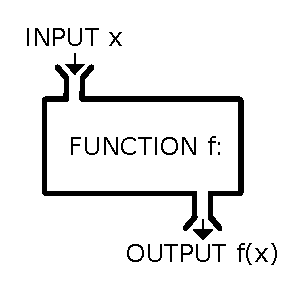
\includegraphics[width=.75\textwidth,keepaspectratio] {Function_machine2.pdf}
%   https://commons.wikimedia.org/wiki/File:Function_machine2.svg
%   \caption{Matrix Entries}
  \end{figure}
\end{frame}

\begin{frame}{What is Functional Programming?}

{\large Functional programming represents a programming paradigm in which the computations are evaluated by mathematical functions. The paradigm avoids changing state and using mutable data.~\footcite{Nita2019}%\footnote[frame]{Haskell Quick Syntax Reference}
}   


{\normalsize Functional programming 代表一種以數學函式來計算的程式設計法。這種設計法避免狀態改變及使用可變資料。
}

% 函數式編程代表一種編程計算被評估的範式 數學函數。範式避免改變 狀態和使用可變數據
% Functional programming 代表一種以數學函式來計算的程式設計法。這種設計法避免狀態改變及使用可變資料
\end{frame}

\begin{frame}{Huh???}
    
  \begin{figure}
  
\includegraphics[width=.75\textwidth,keepaspectratio] {huh.jpg}
%   confused nick young high resolution
  \end{figure}
\end{frame}


%%%%%%%%%%%%%%%%%%%%%%%%%%%%%%%%%%%%%%%%%%%%%%%%%%%%%

\begin{frame}{What is Functional Programming?}
In a nutshell,
\Huge{
NO SIDE EFFECTS!}
\end{frame}

%%%%%%%%%%%%%%%%%%%%%%%%%%%%%%%%%%%%%%%%%%%%%%%%%%%%%


\begin{frame}[fragile]{What is Side Effects?}

\begin{overlayarea}{\linewidth}{.8\textheight}
% https://tex.stackexchange.com/a/271249

\begin{onlyenv}<1->
\begin{lstlisting}[language=JavaScript]
var x = 2;

console.log(x) // 2

function add2(){
    x = x + 2;
}
\end{lstlisting}
\end{onlyenv}

\begin{onlyenv}<2->
\begin{lstlisting}[language=JavaScript,firstnumber=8]
add2();

console.log(x); // 4
\end{lstlisting}
\end{onlyenv}

\onslide<3->{{\huge Not functional, but how to fix it?}}

\end{overlayarea}  
    
\end{frame}


%%%%%%%%%%%%%%%%%%%%%%%%%%%%%%%%%%%%%%%%%%%%%%%%%%%%%

\begin{frame}[fragile]{Let it be Functional}

\begin{overlayarea}{\linewidth}{.8\textheight}
% https://tex.stackexchange.com/a/271249

\begin{onlyenv}<1->
\begin{lstlisting}[language=JavaScript]
var x = 2;

console.log(x) // 2

function add2(y: number){
    return y + 2;
}
\end{lstlisting}
\end{onlyenv}

\begin{onlyenv}<2->
\begin{lstlisting}[language=JavaScript,firstnumber=8]
add2(x);

console.log(x); // 2
\end{lstlisting}
\end{onlyenv}

\onslide<3->{{\huge No side effects}ヽ(o^$\bigtriangledown$^o)ノ}

\end{overlayarea}  

\end{frame}
%%%%%%%%%%%%%%%%%%%%%%%%%%%%%%%%%%%%%%%%%%%%%%%

\begin{frame}{Other Characteristics of Functional Programming}

{\Huge Everything is function}

\pause
\large
Functions are first class

\pause
can be passed, returned, assigned, etc..

\bigskip 
\pause
{\Huge Data is immutable}

\pause
State cannot change after creation
    
\end{frame}
%%%%%%%%%%%%%%%%%%%%%%%%%%%%%%%%%%%%%%%%%%%%%%%


\plain{{\Huge Questions?}\\\bigskip 
  \begin{figure}
  \centering
  
\includegraphics[width=.35\textwidth,keepaspectratio] {slido_coscup22-fp.pdf}
  \caption{sli.do/coscup22-fp}
  \end{figure}
}

%%%%%%%%%%%%%%%%%%%%%%%%%%%%%%%%%%%%%%%%%%%%%%%

\section{Let's Make a Bulls and Cows Solver}

\begin{frame}{What is Bulls and Cows}

\[\text{{\Huge 1A2B}}\]

\begin{itemize}
    \item Secret number: 4271
    \item Opponent's try: 1234
    \item Answer: 1A2B (1 bull and 2 cows)\\If the matching digits are in their right positions, they are "bulls", if in different positions, they are "cows".
\end{itemize}

\end{frame}
%%%%%%%%%%%%%%%%%%%%%%%%%%%%%%%%%%%%%%%%%%%%%%%

\begin{frame}{Bulls and Cows Example}
Secret number: \texttt{9527}
\begin{itemize}[<+(1)->]
    \item I guess ``34\underline{72}'' $\rightarrow$ 0A2B
    \item I guess ``\underline{2}064'' $\rightarrow$ 0A1B
    \item I guess ``\alert{9}\underline{7}48'' $\rightarrow$ 1A1B
    \item I guess ``1\alert{5}4\alert{7}'' $\rightarrow$ 2A0B
    \item I guess ``134\underline{9}'' $\rightarrow$ 0A1B
    \item ``9527''
\end{itemize}

Source: \url{https://github.com/smailzhu/Bulls-and-Cows-Solver}

% A:? 1
% B:? 1
% A:? 2
% B:? 0
% A:? 0
% B:? 1
% "9527"

\end{frame}

%%%%%%%%%%%%%%%%%%%%%%%%%%%%%%%%%%%%%%%%%%%%%%%
\subsection{Flow Chart}
\begin{frame}{Flow Chart}
    
\centering

%\resizebox{!}{.8\textheight}{% if required
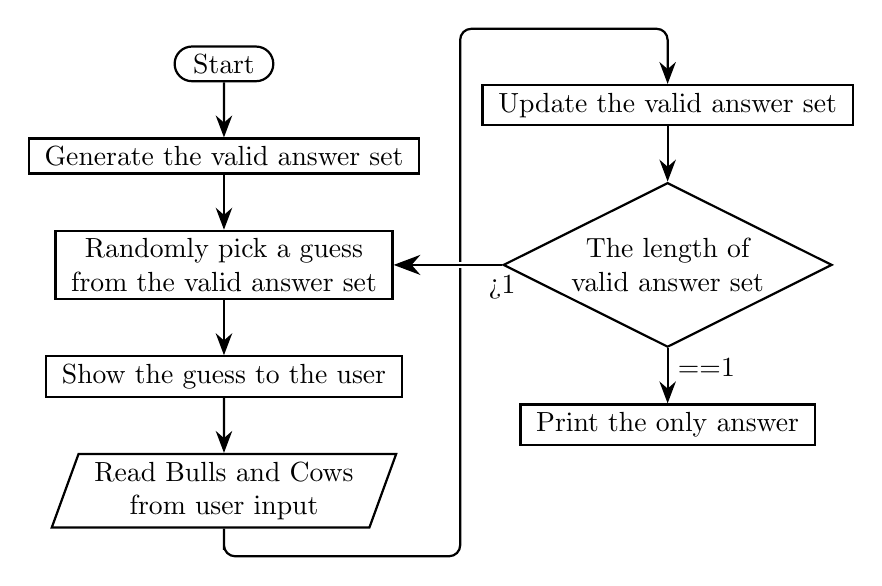
\begin{tikzpicture}[
node distance= 7mm and 12 mm,
     start chain = going below,
     base/.style = {draw, thick, align=center, 
                    inner ysep=1mm, inner xsep=2mm,
                    join=by arrow, on chain}, % 
startstop/.style = {base, rounded rectangle},
       io/.style = {trapezium, base,
                    trapezium left angle=70, trapezium right angle=110},
  process/.style = {base},
 decision/.style = {diamond, aspect=2, base, inner xsep=0pt},
    arrow/.style = {-{Stealth[scale=1.2]}, rounded corners, thick}
                    ]
 % main
\node (start)   [startstop] {Start};
\node (box1)    [process]   {Generate the valid answer set};
\node (box2)    [process]   {Randomly pick a guess\\from the valid answer set};
\node (box3)    [process]   {Show the guess to the user};
\node (io1)     [io]        {Read Bulls and Cows\\from user input};
\node (below_io1) [coordinate, below=3.5mm of io1, reset join] {};  %% Coordinate on right and middle
% \node (box4)    [process, right=of io1.east |- start,reset join] {$X \gets X+1$};
\node (branch1)    [decision, right=1.5 of io1.east |- box2, reset join]  {The length of\\valid answer set};

\node (box4)    [process, above=of branch1.north, reset join]   {Update the valid answer set};
\node (above_box4) [coordinate, above=of box4, reset join] {};  %% Coordinate on right and middle

\draw[arrow] (box4) -- (branch1.north);

% \draw[arrow] (io1.south) -- +(0, -.5) -- + (3,-.5) -- +(3,6.5) -| (box4.north);


\draw[arrow] (io1.south) |- (below_io1) -- ++(3,0) |- (above_box4) -- (box4.north)  ;
\node (box6)    [process, below=of branch1.south, reset join]   {Print the only answer};

\draw[arrow] (branch1.south) node[below right] {==1} -- (box6);
\draw[arrow, draw=white, double=black, double distance=\pgflinewidth, arrows={[black]}] (branch1.west) node[below] {>1} -- (box2.east);
\end{tikzpicture}%
%}
\end{frame}

\subsection{Generate All Valid Answer}
%%%%%%%%%%%%%%%%%%%%%%%%%%%%%%%%%%%%%%%%%%%%%%%%%%%%%%%%%

\begin{frame}
\frametitle{Generate all valid answer}

What is valid answer?
\begin{itemize}
    \item without duplicate digit. e.g. 1234, 9527, \sout{1231}, \sout{6666}
\end{itemize}

\pause
so,
\begin{enumerate}
    % \item Need a function to check list has any duplicate elements
    \item Generate all permutation
    \item Remove invalid permutation
\end{enumerate}
    
\end{frame}

%%%%%%%%%%%%%%%%%%%%%%%%%%%%%%%%%%%%%%%%%%%%%%%%%%%%%



\begin{frame}[fragile]
\frametitle{Check list has any duplicate elements}

\begin{itemize}[<+->]
    \item \texttt{nub} can remove duplicate elements in a list\\ \begin{lstlisting}[language=Haskell,numbers=none]
nub [1,2,3,4,3,2,1,2,4,3,5] -- [1,2,3,4,5]
\end{lstlisting}

    \item make magic happen%
\begin{lstlisting}[language=Haskell]
{- check if list has duplicate element
 -
 - hasDuplicates [1,2,3,4] == False
 - hasDuplicates [1,2,3,1] == True -}
 
hasDuplicates :: Eq a => [a] -> Bool
hasDuplicates xs = length (nub xs) /= length xs
\end{lstlisting}
\end{itemize}
    
\end{frame}

%%%%%%%%%%%%%%%%%%%%%%%%%%%%%%%%%%%%%%%%%%%%%%%%%%%%%


\begin{frame}[fragile]
\frametitle{Generate all valid answer}
\begin{enumerate}[<+->]
    \item \texttt{replicateM}: replicateM n act performs the action act n times, and then returns the list of results:\\ \begin{lstlisting}[language=Haskell,numbers=none]
replicateM 4 [1,2,3,4,5]
--[[1,1,1,1],[1,1,1,2],...,[5,5,5,4],[5,5,5,5]]
    \end{lstlisting}
    \item Remove invalid permutation\\ \begin{lstlisting}[language=Haskell,numbers=none]
filter (>5) [1,2,3,4,5,6,7,8] -- [6,7,8]
filter (\x -> length x > 2) ["aaaa","bbb","cc"] -- ["aaaa", "bbb"]
    \end{lstlisting}
    \item Combine them \begin{lstlisting}[language=Haskell,numbers=none]
allAnswer n x = filter (\x -> not $ hasDuplicates x) $ replicateM n x
allAnswer 4 [0..9] -- [[1,2,3,4],[1,2,3,5],...,[6,7,8,9]]
    \end{lstlisting}
    
\end{enumerate}

\end{frame}

%%%%%%%%%%%%%%%%%%%%%%%%%%%%%%%%%%%%%%%%%%%%%%%%%%%%%


\subsection{How to Count Bulls}

%%%%%%%%%%%%%%%%%%%%%%%%%%%%%%%%%%%%%%%%%%%%%%%%%%%%%

\begin{frame}[fragile]
{Before We Count Bulls}
    \begin{itemize}[<+->]
    \item What is \texttt{(x:xs)} ?\\ \begin{lstlisting}[language=Haskell,numbers=none]
sum :: [Int] -> Int 
sum [] = 0 
sum (x:xs) = x + sum xs 
    \end{lstlisting}
    
    \item For example: \texttt{sum [1,2,3]}\\
    \begin{description}%[\null]
        \item \texttt{sum [1,2,3] = 1 + sum [2,3]}
        \item \texttt{sum [2,3]   = 2 + sum [3]}
        \item \texttt{sum [3]     = 3 + sum []}
        \item \texttt{sum []      = 0}
    \end{description}
%     \begin{lstlisting}[language=Haskell,numbers=none]
% sum [1,2,3] = 1 + sum [2,3]
% sum [2,3]   = 2 + sum [3]
% sum [3]     = 3 + sum []
% sum []      = 0
%     \end{lstlisting}
    \end{itemize}
\end{frame}

%%%%%%%%%%%%%%%%%%%%%%%%%%%%%%%%%%%%%%%%%%%%%%%%%%%%%

\begin{frame}[fragile]
\frametitle{Count Bulls}
\begin{itemize}%[<+->]
    \item What is \texttt{(x:xs)} ?\\ \begin{lstlisting}[language=Haskell,numbers=none]
sum :: [Int] -> Int 
sum [] = 0 
sum (x:xs) = x + sum xs 
    \end{lstlisting}
    
    \item How to count Bulls?\\
     \begin{lstlisting}[language=Haskell]
checkA :: Eq a => [a] -> [a] -> Int
checkA [] [] = 0
checkA (x:xs) (y:ys)
          | x == y    = 1 + (checkA xs ys)
          | otherwise = checkA xs ys
    \end{lstlisting}
\end{itemize}
    
\end{frame}

%%%%%%%%%%%%%%%%%%%%%%%%%%%%%%%%%%%%%%%%%%%%%%%%%%%%%

\begin{frame}[fragile]
\frametitle{Count Bulls}
\begin{itemize}%[<+->]
    \item How to count Bulls?\\
     \begin{lstlisting}[language=Haskell]
checkA :: Eq a => [a] -> [a] -> Int
checkA [] [] = 0
checkA (x:xs) (y:ys)
          | x == y    = 1 + (checkA xs ys)
          | otherwise = checkA xs ys
    \end{lstlisting}
    
    \item Example\\ 
%     \begin{lstlisting}[language=Haskell,numbers=none]
% checkA [4,2,7,1] [1,2,3,4]
% 4\=1 -> checkA [2,7,1] [2,3,4]
% 2==2 -> 1 + checkA [7,1] [3,4]
% 7\=3 -> checkA [1] [4]
% 1\=4 -> checkA [] []
%     \end{lstlisting}
\begin{description}[<+->]
    \item \texttt{checkA [\alert{4},2,7,1] [\alert{1},2,3,4]}
    \item \texttt{4\textbackslash=1 -> checkA [\alert{2},7,1] [\alert{2},3,4]}
    \item \texttt{2==2 -> 1 + checkA [\alert{7},1] [\alert{3},4]}
    \item \texttt{7\textbackslash=3 -> checkA [\alert{1}] [\alert{4}]}
    \item \texttt{1\textbackslash=4 -> checkA [] []}
\end{description}
    
\end{itemize}
    
\end{frame}



\plain{%{\Huge Questions?}\\\bigskip 
  \begin{figure}
  \centering
  
\includegraphics[width=.35\textwidth,keepaspectratio] {rainbow_cat.pdf}
%   \caption{sli.do/coscup22-fp}
  \end{figure}
}


%%%%%%%%%%%%%%%%%%%%%%%%%%%%%%%%%%%%%%%%%%%%%%%

\subsection{How to Count Cows}

%%%%%%%%%%%%%%%%%%%%%%%%%%%%%%%%%%%%%%%%%%%%%%%%%%%%%%%%%
\begin{frame}[fragile]
\frametitle{Before We Count Cows}
\begin{enumerate}[<+->]
    \item Subtract\\%
    \begin{lstlisting}[language=Haskell,numbers=none]
subtract 3 5 -- 2    
subtract 6 3 -- -3
    \end{lstlisting}
    \item Check if element in a list\\%
    \begin{lstlisting}[language=Haskell,numbers=none]
elem 1 [1,2,3,4,5] -- True
elem 14 [1..10] -- False
    \end{lstlisting}
    
    \item Count elements in a list\\%
    \begin{lstlisting}[language=Haskell,numbers=none]
filter (>5) [1,2,3,4,5,6,7,8] -- [6,7,8]
length [6,7,8] -- 3
length $ filter (>5) [1..8] -- 3
    \end{lstlisting}
    
    \item Map (higher-order function)\\%
    \begin{lstlisting}[language=Haskell,numbers=none]
map square [1, 2, 3, 4, 5] -- [1, 4, 9, 16, 25]
    \end{lstlisting}
\end{enumerate}
    
\end{frame}


%%%%%%%%%%%%%%%%%%%%%%%%%%%%%%%%%%%%%%%%%%%%%%%%%%%%%

\begin{frame}[fragile]
\frametitle{Magic to Count Cows}


\begin{overlayarea}{\linewidth}{.8\textheight}
% https://tex.stackexchange.com/a/271249

    \begin{enumerate}
  \setlength\itemsep{0em}
% \begin{onlyenv}<1->
    \item Before we count Cows\\
    \begin{lstlisting}[language=Haskell,numbers=none]
elem 1 [1,2,3,4,5] -- True
map square [1..5] -- [1,4,9,16,25]
    \end{lstlisting}
% \end{onlyenv}
% \begin{onlyenv}<2->
\item[]<2->%
    \begin{lstlisting}[language=Haskell,numbers=none]
length $ filter (>5) [1..8] -- 3
    \end{lstlisting}
% \end{onlyenv}


% \begin{onlyenv}<1->
    \item Count the number of same elements in two lists\\
     \begin{lstlisting}[language=Haskell,numbers=none]
f1 xs ys = map (\y -> elem y xs) ys 
f1 [2,3,4] [5,2,4] -- [False,True,True]
-- map (\y -> elem y [2,3,4]) [5,2,4]
    \end{lstlisting}
% \end{onlyenv}
% \begin{onlyenv}<2->
\item<2->[]%
     \begin{lstlisting}[language=Haskell,numbers=none]
f2 xs ys = length $ filter (True==) $ f1 xs ys
f2 [2,3,4] [5,2,4] -- 2
-- length $ filter (True==) [False,True,True]
    \end{lstlisting}
% \end{onlyenv}

    \end{enumerate}
\end{overlayarea}
        
\end{frame}


%%%%%%%%%%%%%%%%%%%%%%%%%%%%%%%%%%%%%%%%%%%%%%%%%%%%%


\begin{frame}[fragile]
\frametitle{Let's Count Cows}
    \begin{enumerate}\item Count the number of same elements in two lists\\
     \begin{lstlisting}[language=Haskell,numbers=none]
f1 xs ys = map (\y -> elem y xs) ys 
f1 [2,3,4] [5,2,4] -- [False,True,True]
-- map (\y -> elem y [2,3,4]) [5,2,4]

f2 xs ys = length $ filter (True==) $ f1 xs ys
f2 [2,3,4] [5,2,4] -- 2
-- length $ filter (True==) [False,True,True]
    \end{lstlisting}
        
    \item How to count cows?\\
     \begin{lstlisting}[language=Haskell,numbers=none]
checkAB :: Eq a => [a] -> [a] -> (Int, Int)
checkAB xs ys = (a_num, b_num)
  where a_num = checkA xs ys
        b_num = subtract a_num $ length $ filter (True==) $ map (\y -> elem y xs) ys
    \end{lstlisting}
    \end{enumerate}
\end{frame}



%%%%%%%%%%%%%%%%%%%%%%%%%%%%%%%%%%%%%%%%%%%%%%%%%%%%%


\plain{{\Huge Questions?}\\\bigskip 
  \begin{figure}
  \centering
  
\includegraphics[width=.35\textwidth,keepaspectratio] {slido_coscup22-fp.pdf}
  \caption{sli.do/coscup22-fp}
  \end{figure}
}


%%%%%%%%%%%%%%%%%%%%%%%%%%%%%%%%%%%%%%%%%%%%%%%%%%%%%

\subsection{Function Composition}


%%%%%%%%%%%%%%%%%%%%%%%%%%%%%%%%%%%%%%%%%%%%%%%%%%%%%


\begin{frame}{Function Composition}

     
     
\begin{columns}
\begin{column}{0.4\textwidth}
   
     \begin{equation*}
         g\circ f(x)=g(f(x))
     \end{equation*}
     
\end{column}
\begin{column}{0.6\textwidth}  %%<--- here
    
  \begin{figure}
  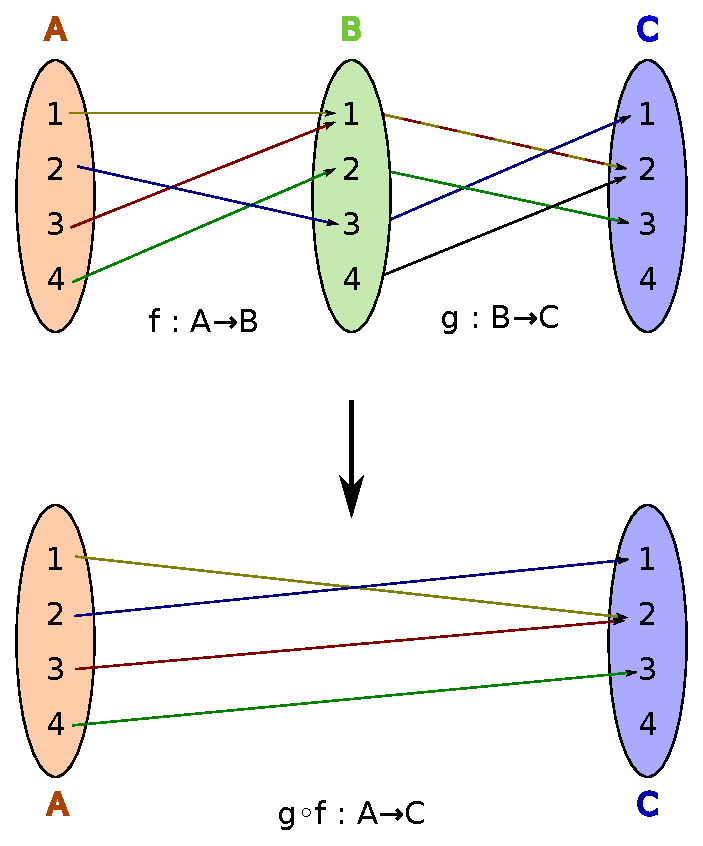
\includegraphics[width=.75\textwidth,keepaspectratio] {Example_for_a_composition_of_two_functions.pdf}
%   confused nick young high resolution
    \caption{Example for a composition of two functions~\footnote[frame]{From wikimedia commons by Stephan Kulla}}
  \end{figure}
\end{column}

\end{columns}
  
    
\end{frame}

%%%%%%%%%%%%%%%%%%%%%%%%%%%%%%%%%%%%%%%%%%%%%%%%%%%%%

\begin{frame}{Function Composition}
  \begin{figure}
  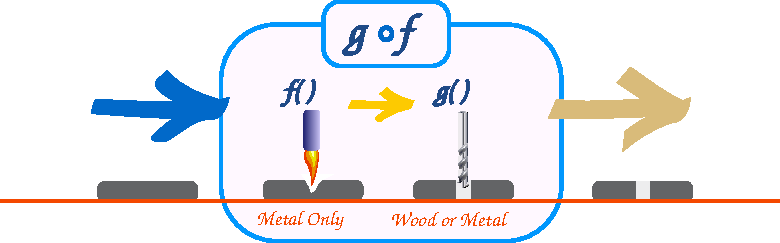
\includegraphics[width=\textwidth,keepaspectratio] {function-composition-c.pdf}
%   confused nick young high resolution
    \caption{Composition of Functions~\footnote{https://www.mathsisfun.com/sets/functions-composition.html}}
  \end{figure}
  
\end{frame}

%%%%%%%%%%%%%%%%%%%%%%%%%%%%%%%%%%%%%%%%%%%%%%%%%%%%%

\begin{frame}[fragile]
\frametitle{Update Valid Answer}
    
     \begin{lstlisting}[language=Haskell,numbers=none]
{- Update answer pool
 - choose the solutions which match the rules base on the test
 -}
updateAnswers :: Eq a => [[a]] -> [a] -> (Int, Int) -> [[a]]
updateAnswers ans test rules
        = filter ((rules==).(checkAB test)) ans
    \end{lstlisting}
\end{frame}


%%%%%%%%%%%%%%%%%%%%%%%%%%%%%%%%%%%%%%%%%%%%%%%%%%%%%

\plain{{\Huge Questions?}\\\bigskip 
  \begin{figure}
  \centering
  
\includegraphics[width=.35\textwidth,keepaspectratio] {slido_coscup22-fp.pdf}
  \caption{sli.do/coscup22-fp}
  \end{figure}
}

\end{document}
